\subsection{Optymalizacja obliczeń matematycznych}
\thispagestyle{empty}
\par\indent

Renderując dużą ilość niewielkich obiektów należy pamiętać o optymalizacji obliczeń jeszcze przed samym renderingiem sceny. Obliczenia na liczbach zmiennoprzecinkowych oraz macierzach zużywają znaczącą ilość czasu procesora. 

\subsubsection{Program początkowy}
\thispagestyle{empty}
\par\indent

Już na tym etapie można zyskać znaczną poprawę czasu renderowania.  W tym przypadku wyświetlanych będzie 20000 sześcianów, które obracane są względem osi pionwej. Dane wierzchołków (położenie oraz kolor) dla wszystkich sześcianów są takie same. Informacje o przesunięciu oraz obrocie sześciany przekazywane są do wbudowanego w OpenGL procesu renderującego.

\lstinputlisting[language=c++,caption=Algorytm dynamicznie renderujący sześciany]{sources/unoptimized_rendering_loop.cpp}
\lstinputlisting[language=c++,caption=Algorytm obliczania docelowego położenia każdego wierzchołka]{sources/basic_vertex_shader.shader}
\lstinputlisting[language=c++,caption=Algorytm obliczenia koloru wierzchołka]{sources/basic_fragment_shader.shader}

Jak widzimy wszystkie obliczenia powtarzane są dla każdego sześcianu. Taka struktura programu owocuje długim czasem renderowania każdej klatki który trwa średnio 0.6 sekundy. Daje to około 16 klatek w cięgu 10 sekund.

\begin{figure}[h]
	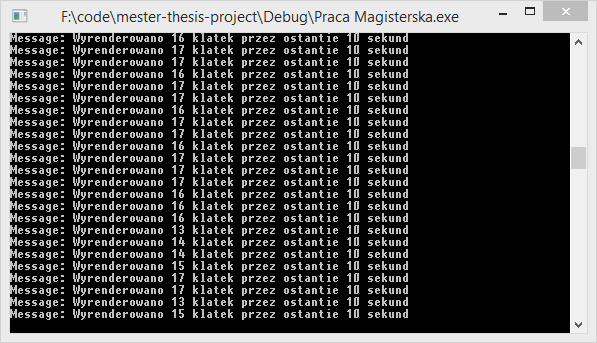
\includegraphics[width=\textwidth]{images/optimized0_console}
	\caption{Inforamcje diagnostyczne}
\end{figure}


\subsubsection{Usunięcie zbędnych obliczeń na macierzach}
\thispagestyle{empty}
\par\indent

Warto tutaj zauważyć, że macierz projekcji oraz widoku jest taka sama dla każdego wierzchołka. Może zmienić się ona co najwyżej raz dla każdej klatki. Dlatego warto przemieść obliczanie ich ilorazu na początek pętli renderującej klatkę. Nie wprowadzi to potrzeby zmian w obliczeniach per wierzchołek.

\lstinputlisting[language=c++,caption=Pętla renderująca]{sources/optimized_matrix_operations.cpp}

\begin{figure}[h]
	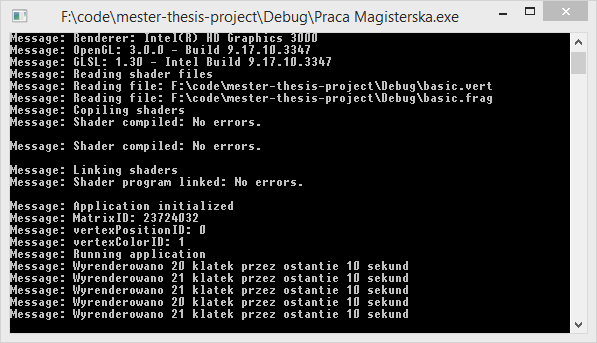
\includegraphics[width=\textwidth]{images/optimized1_console}
	\caption{Inforamcje diagnostyczne}
\end{figure}


\subsubsection{Przeniesienie obliczeń do Shadera}
\thispagestyle{empty}
\par\indent

Kolejnym krokiem w optymalizacji obliczeń jest przeniesienie operacji na macierzach do jednostek obliczeniowych znajdujących się na  karcie graficznej. Jak zostało wspomniane w poprzednich rozdziałach GPU został zaprojektowany do wykonywania obliczeń zmiennoprzecinkowych. Dodatkowo odciąży to jednostkę CPU i skróci czas wykonywania kolejnych obrotów pętli.

Aby tego dokonać należy zmodyfikować vertex shader aby akceptował dodatkowy parametr oraz wykonywał niezbędne obliczenia.

\lstinputlisting[language=c,caption=Vertex Shader]{sources/vertex_shader_with_additional_matrix.shader}

Następnie należy odpowiednio zmodyfikować pętle renderrujące sześciany.

\lstinputlisting[language=c,caption=Pętla renderująca]{sources/rendering_loop_wo_matrix_operations.cpp}

Wzrost wydajności znowu jest znaczący. Czas wymagany do wykonania wszystkich obliczeń per klatka zmniejszył się do 0.34 sekundy. Pozwala to na wyświetlenie średnio 28 klatek w czasie 10 sekund.

\begin{figure}[h]
	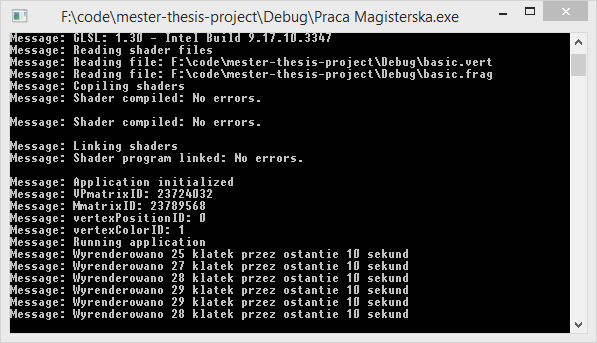
\includegraphics[width=\textwidth]{images/optimized2_console}
	\caption{Inforamcje diagnostyczne}
\end{figure}

\subsubsection{Wnioski}
\thispagestyle{empty}
\par\indent

Dzięki powyższym zabiegom otrzymaliśmy czerokrotny wzrost wydajności. Czas renderowania jednej klatki został drastycznie zmniejszony. Warto tuatj zauwazyć, iż dobór miejsca wykonywania operacji matematycznych jest niezwykle ważny. Przede wszystkiem nie powinny znajdować się one w pętlach jeżeli nie jest to koneiczne. Gdy istneije taka możliwość powinny być one wykonywane przez jednostkę specjalnie zaprojektowaną do tego celu, dla liczb zmiennoprzecinkowych GPU, a dla stałoprzecinkowych CPU.

Proces optymalizacji tego fragmentu kodu można uznać jako niepełny ponieważ znajjdują się w nim operacje macierzowe wykonywane przez CPU. Jendka nie można ich zlikwidować ponieważ renderowane obiekty tworzone są dynamicznie. Proces przenoszenia operacji tworzenia  macierzy modelu do jednostki GPU nie dałby oczekiwanych rezultatów. Argumentem za tym ztojącym jest fakt iż dla każdego wierzchołka dana macierz byłaby tworzona niealeznie. Co za tym idzie wzrósłby narzut pamięciowy oraz obliczeniowy.
